    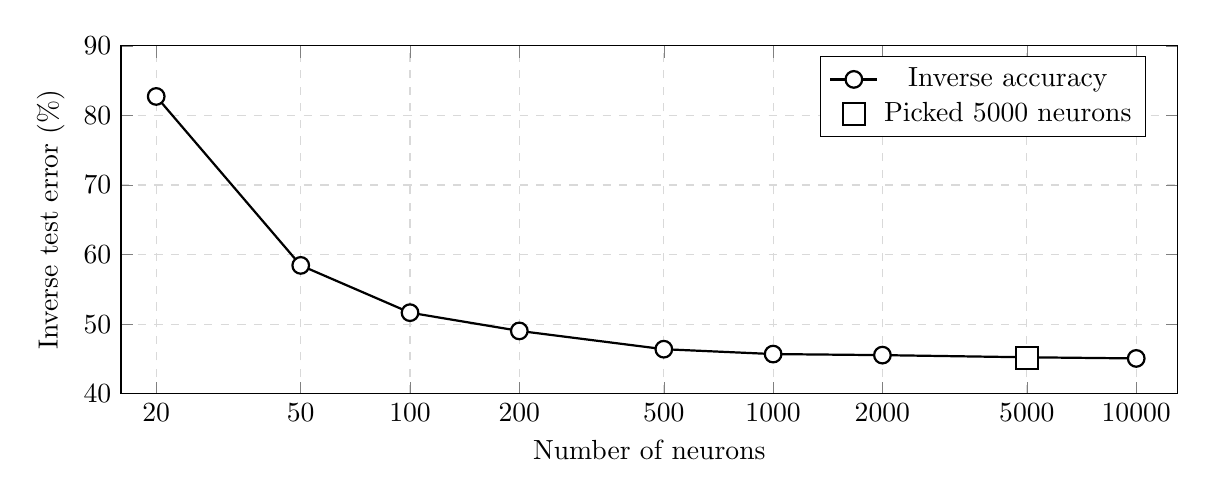
\begin{tikzpicture}
    \begin{axis}[
        width=15cm,
        height=6cm,
        xlabel={Number of neurons},
        ylabel={Inverse test error (\%)},
        grid=major,
        grid style={dashed,gray!30},
        xmode=log,
        log basis x=10,
        xmin=16, xmax=13000,
        xtick={20,50,100,200,500,1000,2000,5000,10000},
        xticklabels={20,50,100,200,500,1000,2000,5000,10000},
        ymin=40, ymax=90,
        ytick={40, 50, 60, 70, 80, 90},
        legend pos=north east,
        mark size=3pt,
        % line width=1.5pt,
        every axis plot/.append style={thick},
        title style={font=\Large\bfseries},
        tick label style={font=\normalsize},
        legend style={font=\normalsize}
    ]
    % Data points
    \addplot[
        color=black,
        mark=*,
        mark options={fill=white}
    ] coordinates {
        (20, 82.723)
        (50, 58.439)
        (100, 51.647)
        (200, 49.023)
        (500, 46.396)
        (1000, 45.696)
        (2000, 45.544)
        (5000, 45.234)
        (10000, 45.07)
    };
    % Highlight the best performance
    \addplot[
        color=black,
        mark=square*,
        mark size=4pt,
        mark options={fill=white},
        only marks
    ] coordinates {
        (5000, 45.168)
    };
    \legend{Inverse accuracy, Picked 5000 neurons}
    % Add annotations for key points
    % \node[pin=45:{Best: 0.45144}] at (axis cs:5000,0.45168) {};
    \end{axis} 
    \end{tikzpicture}